\documentclass[11pt, fleqn]{article}

\usepackage[usenames,dvipsnames,svgnames,table]{xcolor}
\usepackage{amsmath}
\usepackage{amsfonts}
\usepackage[margin=1in]{geometry} % To set the margin widths
\usepackage{graphicx}
\usepackage{listings}
\usepackage{multirow}
\usepackage{tabularx}
\usepackage{varioref}
\usepackage[noabbrev,capitalize]{cleveref}
\usepackage[group-separator={,}]{siunitx}
\usepackage{subcaption}
\usepackage{titlesec}
\usepackage{lscape}
\usepackage{bm}
\usepackage{chngpage}
\usepackage[titletoc,toc,title]{appendix}

\renewcommand\thesection{\arabic{section}}
\renewcommand\thesubsection{\thesection\alph{subsection}}

\lstset{
  frame=single,
  basicstyle=\ttfamily,% print whole listing small
  language=R,
  aboveskip=3mm,
  belowskip=3mm,
  showstringspaces=false,
  columns=flexible,
  numbers=none,
  commentstyle=\color{ForestGreen},
  stringstyle=\color{Maroon},
  breaklines=true,
  breakatwhitespace=true,
  tabsize=2,
  literate={<-}{{$\gets$}}1 {~}{{$\sim$}}1
}

\sisetup{output-exponent-marker=\textsc{e}}

\setlength{\parskip}{12pt} % Sets a blank line in between paragraphs
\setlength\parindent{0pt} % Sets the indent for each paragraph to zero

\begin{document}

\title{Homework \#1\\
Digital and Algorithmic Marketing (37304-01)}
\author{Brian Chingono, Will Clark, Matthew DeLio, Yoni Sarason, Jonathan Stevens\\
University of Chicago Booth School of Business}

\maketitle

\section{Data Exploration (JS)}

% Note this CDF plot is for customers that did spend at least something
\begin{figure}[!htb]
  \centering
  \caption{CDF of Customer Spending}
  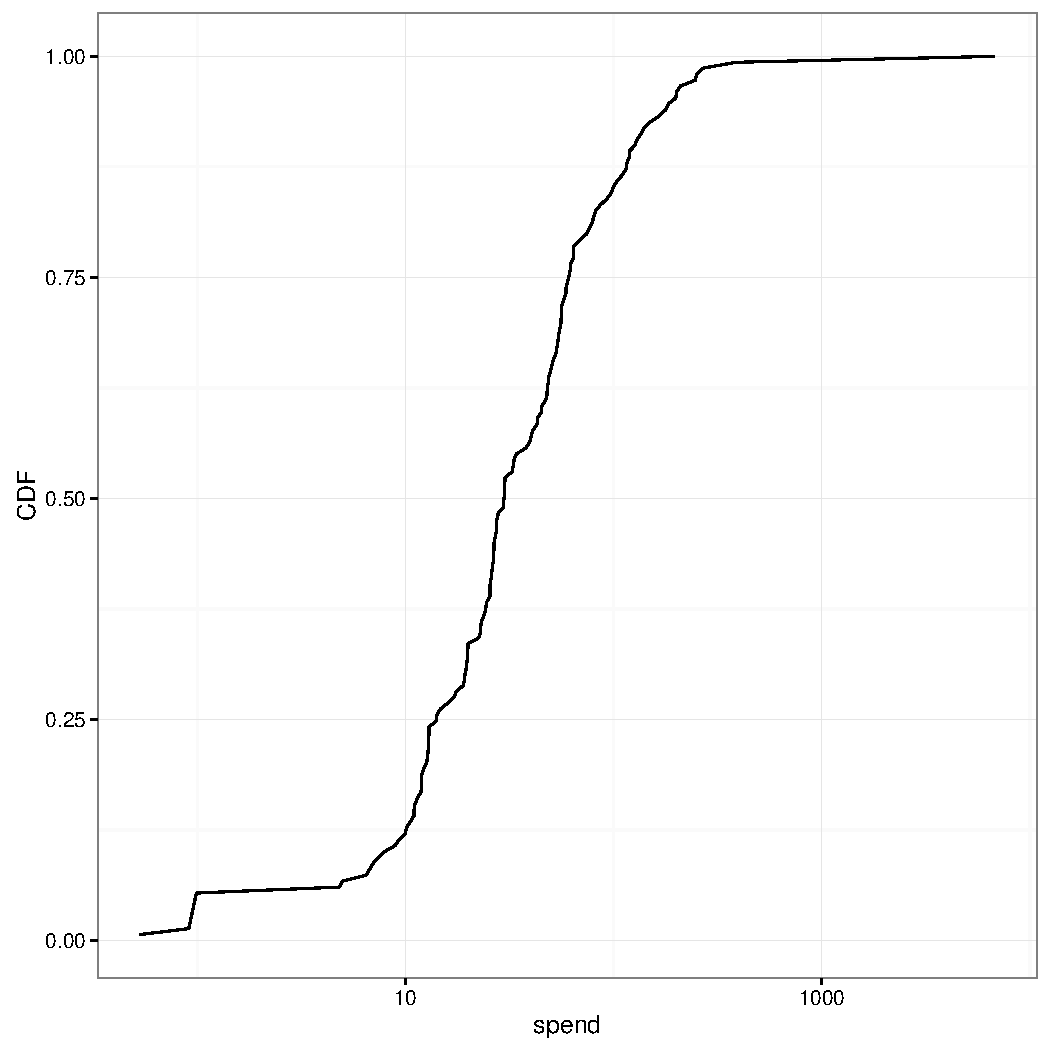
\includegraphics[scale=.5]{cust_spend_cdf.pdf}
  \label{fig:cust_spend_cdf}
\end{figure}

% Again, this is for actual customers that spent something.
% we might want to only include the histogram or cdf.
\begin{figure}[!htb]
  \centering
  \caption{Histogram of Customer Spending}
  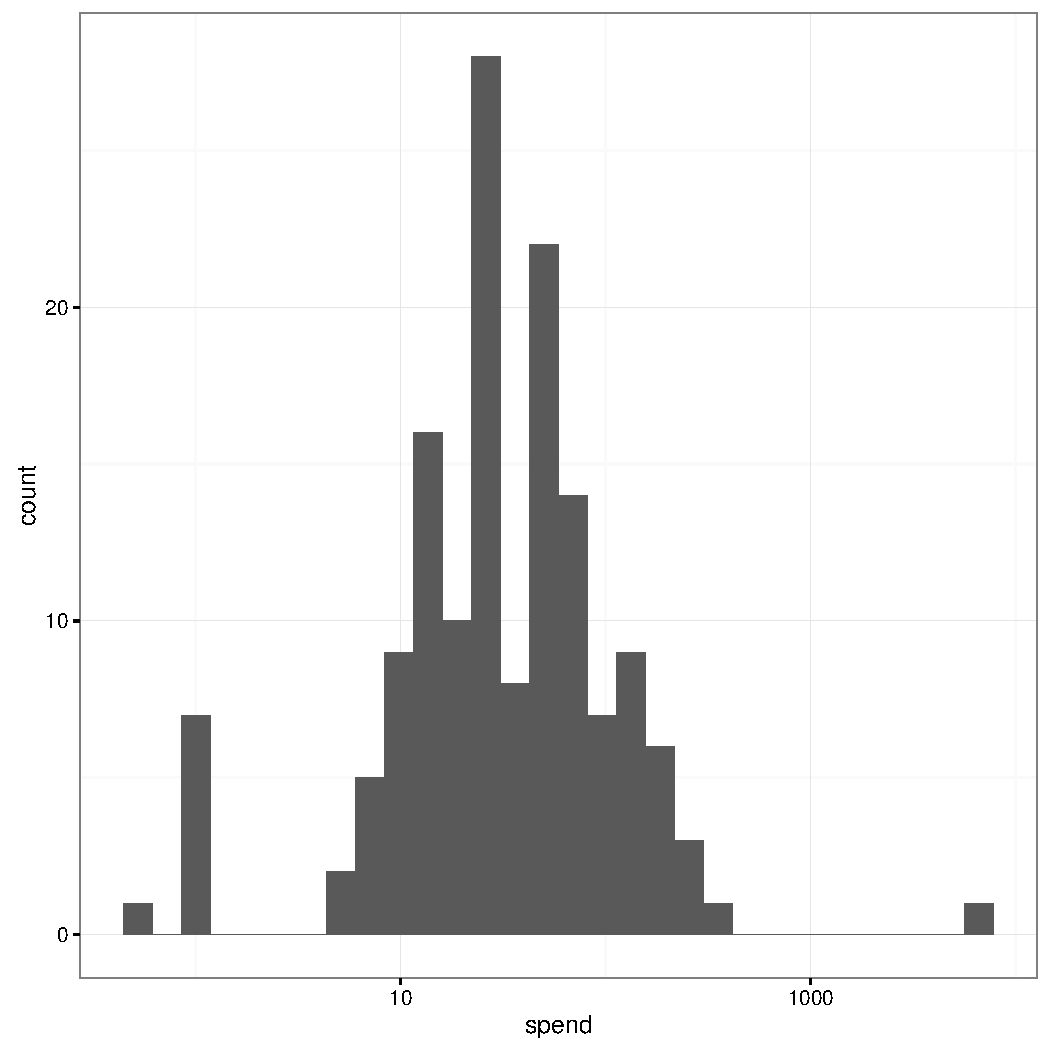
\includegraphics[scale=.5]{cust_spend_hist.pdf}
  \label{fig:cust_spend_hist}
\end{figure}


\section{K-Means Matching (WC)}

Yes. We would use the new DMP. A regression of spend against the explanatory variables shows that the new ecom\_index variable is statistically significant. Moreover, the retail\_index variable is no longer statistically significant after we control for ecom\_index. Therefore, the new DMP provides a variable that allows us to obtain better matches than our original method.

As shown in the chart below, we can obtain a higher maximum profit under the new DMP than under our original method. Under the new DMP, profit is maximized at \$4,413.61 whereas the maximum profit under the old method was \$3,559.14. In both cases, profit is maximized when k-nearest neighbors are set to 3. See \vref{fig:profits}.

\section{K-Nearest-Neighbors Matching (MLD)}

% latex table generated in R 3.2.3 by xtable 1.8-2 package
% Tue Apr 12 03:01:59 2016
\begin{table}[ht]
\centering
\caption{Best matching threshold by explanatory variables} 
\label{tab:series_max}
\begin{tabular}{lrlrrrrr}
  \hline
Series & MatchingThreshold [\$] & Threshold \% & Best NN Choice & Profit [\$] & \% Cust Captured & \% Revenue Captured & \% Cust Matched \\ 
  \hline
Manual & 41.10 & 57.5\% &   7 & 4800.48 & 79.09 & 82.79 & 43.72 \\ 
  AIC & 8.72 & 10\% &   3 & 5028.85 & 82.73 & 85.17 & 51.41 \\ 
  BIC & 35.62 & 55\% &   7 & 4541.70 & 76.36 & 80.04 & 37.67 \\ 
   \hline
\end{tabular}
\end{table}


\begin{figure}[!htb]
  \centering
  \caption{Profits using K-Nearest Neighbors}
  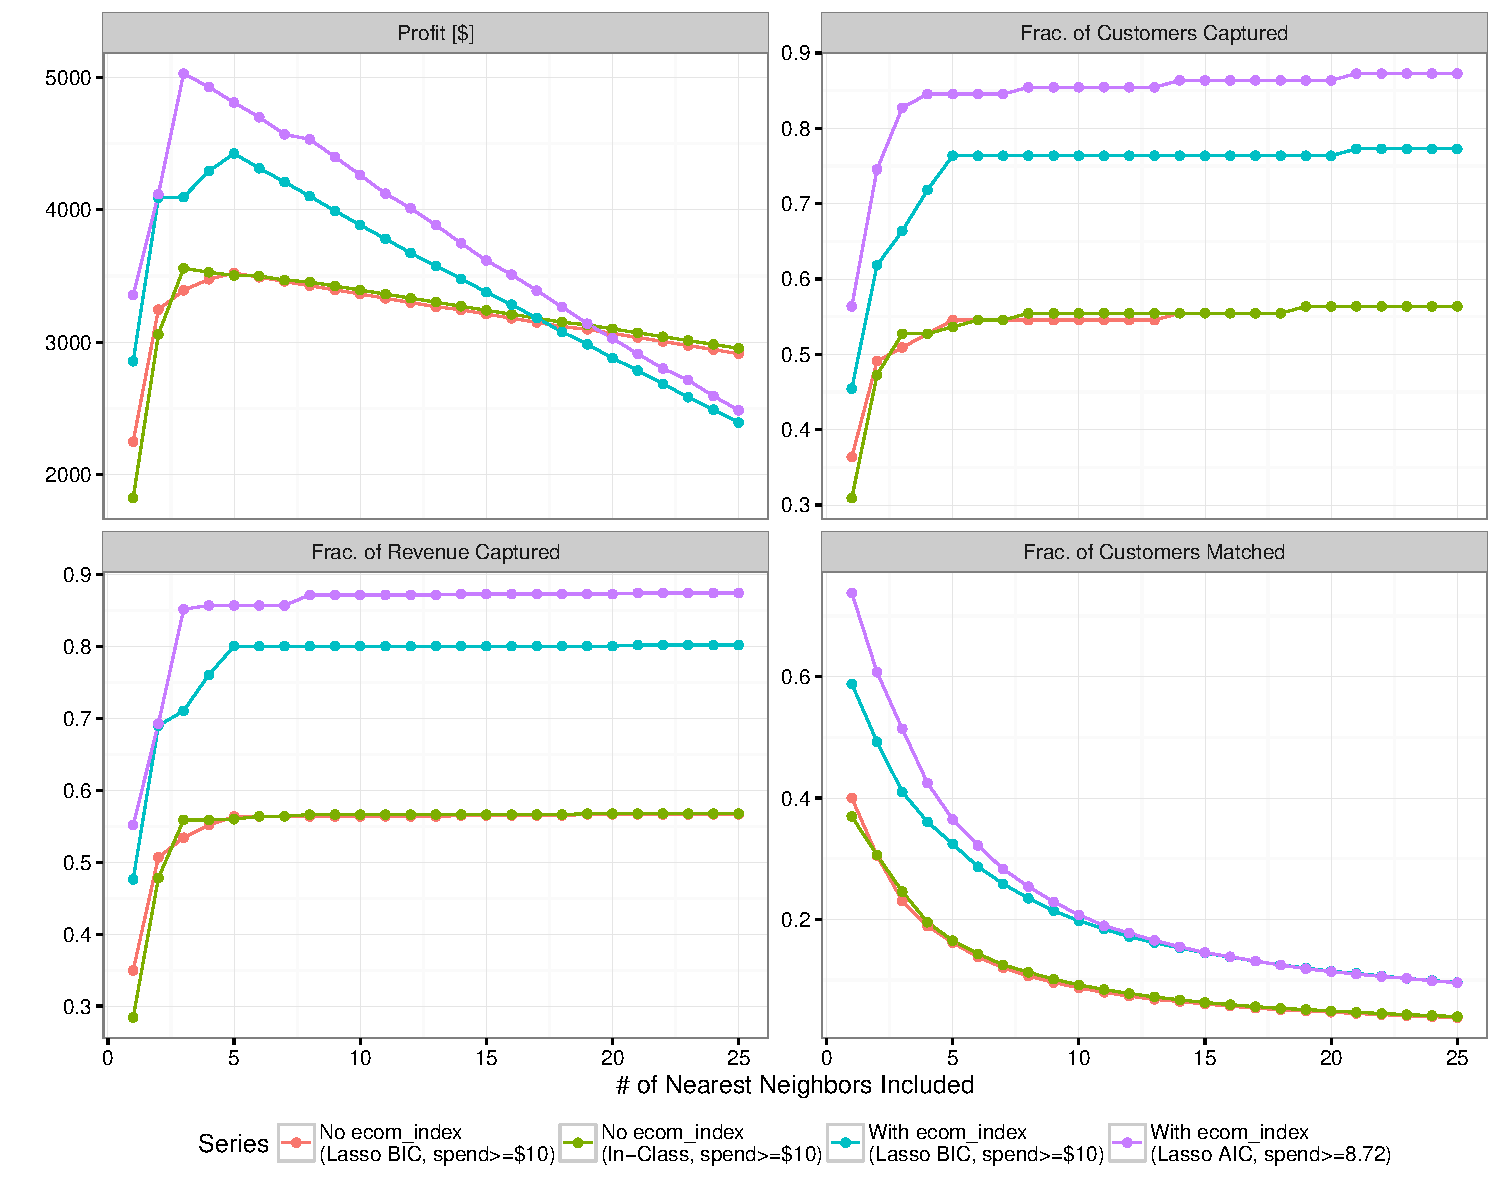
\includegraphics[scale=.75]{profits.pdf}
  \label{fig:profits}
\end{figure}

\section{Targeting the Entire Data Set (BC)} % Question 2

\end{document}

% \input{.tex}

% \begin{figure}[!htb]
%   \centering
%   \caption{}
%   \begin{subfigure}[b]{0.49\textwidth}
%     \caption{}
%     \includegraphics[width=\textwidth]{.pdf}
%     \label{fig:}
%   \end{subfigure}
%   \hfill
%   \begin{subfigure}[b]{0.49\textwidth}
%     \caption{}
%     \includegraphics[width=\textwidth]{.pdf}
%     \label{fig:}
%   \end{subfigure}
% \end{figure}

% \begin{figure}[!htb]
%   \centering
%   \caption{}
%   \includegraphics[scale=.5]{.pdf}
%   \label{fig:}
% \end{figure}